\documentclass[12pt,titlepage]{article}
\usepackage[table]{xcolor}
\usepackage{longtable}
\usepackage[utf8]{inputenc}
%Language of Document Elements like Figure or Table
\usepackage[english]{babel}
\usepackage[bookmarks]{hyperref}
\usepackage{pdfpages}
\usepackage{graphicx}
\usepackage{float}
\usepackage{array}
\usepackage{lipsum} 
\usepackage[justification=centering]{caption}
\usepackage{enumitem}
\usepackage{chngcntr}
\usepackage{lscape}
\usepackage{fancyhdr}
\usepackage{listings}
\usepackage[style=alphabetic, backend=biber]{biblatex}
\usepackage{dafny}
\usepackage{hyperref}
\usepackage{nameref}
\usepackage[margin=1in]{geometry}

%Each Section in a new Page
\let\oldsection\section
\renewcommand\section{\clearpage\oldsection}

%Set space around and between lists
\setlist[enumerate]{noitemsep, topsep=0cm}
\setlist[itemize]{noitemsep, topsep=0cm}

%Figure/Table Numbering style "Section Number.figure counter
\renewcommand{\thefigure}{\arabic{section}.\arabic{figure}}
\renewcommand{\thetable}{\arabic{section}.\arabic{table}}

%Reset figure/table counter after section change
\counterwithin{figure}{section}
\counterwithin{table}{section}

%Syntax Highlighting
%\lstdefinestyle{dafny}{
%	language=dafny, 
%	basicstyle=\normalfont\ttfamily,
%	numbers=left,
%	numberstyle=\scriptsize,
%	stepnumber=1,
%	numbersep=8pt,
%	showstringspaces=false,
%	breaklines=true,
%	frame=lines,
%	backgroundcolor=\color{background}
%}

\colorlet{punct}{red!60!black}
\definecolor{background}{HTML}{EEEEEE}
\definecolor{delim}{RGB}{20,105,176}
\colorlet{numb}{magenta!60!black}

\lstdefinelanguage{json}{
	basicstyle=\normalfont\ttfamily,
	numbers=left,
	numberstyle=\scriptsize,
	stepnumber=1,
	numbersep=8pt,
	showstringspaces=false,
	breaklines=true,
	frame=lines,
	backgroundcolor=\color{background},
	literate=
	*{0}{{{\color{numb}0}}}{1}
	{1}{{{\color{numb}1}}}{1}
	{2}{{{\color{numb}2}}}{1}
	{3}{{{\color{numb}3}}}{1}
	{4}{{{\color{numb}4}}}{1}
	{5}{{{\color{numb}5}}}{1}
	{6}{{{\color{numb}6}}}{1}
	{7}{{{\color{numb}7}}}{1}
	{8}{{{\color{numb}8}}}{1}
	{9}{{{\color{numb}9}}}{1}
	{:}{{{\color{punct}{:}}}}{1}
	{,}{{{\color{punct}{,}}}}{1}
	{\{}{{{\color{delim}{\{}}}}{1}
	{\}}{{{\color{delim}{\}}}}}{1}
	{[}{{{\color{delim}{[}}}}{1}
	{]}{{{\color{delim}{]}}}}{1},
}


%TODO
\newcommand{\todonl}[1]{\newline\textcolor{red}{TODO: #1}\PackageWarning{TODO:}{#1!}}
\newcommand{\todo}[1]{\textcolor{red}{TODO: #1}\PackageWarning{TODO:}{#1!}}

%Set Paragraph indent to null
\setlength{\parindent}{0pt}
% Smaler Table Space
\renewcommand{\arraystretch}{1.5}

\title{Visual Studio Code Integration for the Dafny Language and Program Verifier}
\author{Rafael Krucker, Markus Schaden}
\date{20.02.2017}

\pagestyle{fancy}
\lhead{BA Dafny}
\addbibresource{LITERATURVERZEICHNIS/bibliographie.bib}
\begin{document}
\pagenumbering{Roman} 

% TODO

\includepdf{titlepage/titlepage}


% TODO
%\includepdf[pages={1-}, 
%scale=0.9,pagecommand=\thispagestyle{plain}]{additionals/eigenstaendigkeit}
%\includepdf[pages={1-2}, 
%scale=0.9,pagecommand=\thispagestyle{plain}]{additionals/aufgabenstellung}

\newpage
\tableofcontents
\newpage
\pagenumbering{arabic}


\section{Dafny}
Dafny consists out of 4 different projects. DafnyDriver, DafnyPipleline, DafnyRuntime and the DafnyServer. Most important was the DafnyServer for this project. It had been forked to allow extensions which were merged back into the master branch of Microsoft. 
\subsection{Overview}
Dafny itself does not verify programs, but does the translation into boogie code. Boogie does mostly the same, it can translate the code to different prove engines. Additionally it can be configured to do the verification slightly different. One of the prove engines, which was used for this project is Z3. This engine can verify if a logical formula can be proven. If a prove is found, it can also be viewed, which was important to produce counter examples, were the prove was negated. 
Additionally the DafnyServer is part of Dafny and allows caching and the opportunity to not start a new process for each verification.\newline 
\begin{figure}[H]
	\centering
	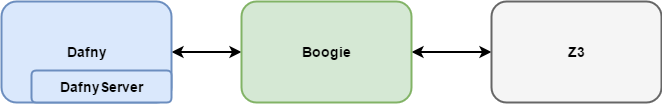
\includegraphics[width=0.8\textwidth]{img/dafny_overview}
	\caption{Interaction between Dafny, Boogie and Z3}
	\label{fig:dafny_overview}
\end{figure}
\subsection{DafnyServer API}
The DafnyServer is a simple console application which allows proofing Dafny source files. To verify documents, they are sent over the standard input. Results are obtained from the standard output. The verification task needs to be in JSON format, see \ref{verificationtaskinterface}, and is sent base64 encoded. By default, the server only supports the verbs verify, quit and selftest. Verbs are sent first, followed by a newline \textbackslash{n}. They may be proceeded by a verification task and the end string \textbf{[[DAFNY-CLIENT: EOM]]}. 
\paragraph{Verb explanation:}
\begin{itemize}
	\item \textbf{verify} needs a verification task and returns the output from the verification
	\item \textbf{quit} stops the server
	\item \textbf{selftest} execute some simple verification.
\end{itemize}
\subsubsection{Verification Task Interface}\label{verificationtaskinterface}
The verification task must use the following structure. \newline
\begin{lstlisting}[language=json,firstnumber=1]
{
  args : [],
  filename : "c:\\DEV\\Dafny\\test.dfy",
  source : "method Main() {  assert 4 < 3; }",
  sourceIsFile : false
}
\end{lstlisting}
\subsubsection{DafnyServer Example}
\textbf{Sample Request}
The base64 encoded string is the verification task from above. 
The following request examples will only show the Dafny program and not how it is sent encoded. 
\begin{lstlisting}[language={},backgroundcolor=\color{background},basicstyle=\scriptsize\ttfamily]
verify
eyJhcmdzIjpbXSwiZmlsZW5hbWUiOiJjOlxcREVWXFxEYWZueVxcdGVzdC5kZnkiLCJzb3VyY2Ui
OiJtZXRob2QgTWFpbigpIHsgIGFzc2VydCAxIDwgMzsgfSIsInNvdXJjZUlzRmlsZSI6ZmFsc2V9
[[DAFNY-CLIENT: EOM]]
\end{lstlisting}
\textbf{Sample Response}
\begin{lstlisting}[language={},backgroundcolor=\color{background},basicstyle=\scriptsize\ttfamily]
Verifying Impl$$_module.__default.Main ...
  [1 proof obligation]  error
c:\DEV\Dafny\test.dfy(1,26): Error: assertion violation
Execution trace:
    (0,0): anon0

Verification completed successfully!
[SUCCESS] [[DAFNY-SERVER: EOM]]
\end{lstlisting}
The result is plain text There is currently no possibility to get a JSON response. Because of that it is needed to parsed and extract the most important parts manually. 
\subsubsection{symbols}
To support refactoring in the Dafny Visual Studio Code plugin, symbol information was needed. All fields, methods and classes inside a file along with their information about position, reference and usage have to be accessible. To support this, the DafnyServer was extended. A new verb "symbols" was introduced. This collects various information about the symbol table of the input file and returns it as JSON. 
\newline\newline
\textbf{Request}
\begin{lstlisting}[language=dafny]
class BankAccountUnsafe {
  var balance: int;
  constructor() modifies this { 
    balance := 10;
  }

  method withdraw(amount: int) 
    modifies this
  requires amount >= 0 {   
    balance := balance - amount; 
  } 
}   

method test() { 
  var a := new BankAccountUnsafe(); 
  a.withdraw(9);  
}   
\end{lstlisting}
\textbf{Response}
\begin{lstlisting}[language=json,firstnumber=1]
[
  ....
  {
    "Call" : null,
    "Column" : 3,
    "EndColumn" : null,
    "EndLine" : null,
    "EndPosition" : null,
    "Ensures" : [],
    "Line" : 3,
    "Module" : "_module",
    "Name" : "_ctor",
    "ParentClass" : "BankAccountUnsafe",
    "Position" : 49,
    "References" : [{
        "Column" : 12,
        "Line" : 15,
        "MethodName" : "test",
        "Position" : 265,
        "ReferencedName" : "_ctor"
      }
    ],
    "Requires" : [],
    "SymbolType" : "Method"
  }, {
    "Call" : null,
    "Column" : 9,
    "EndColumn" : null,
    "EndLine" : null,
    "EndPosition" : null,
    "Ensures" : [],
    "Line" : 6,
    "Module" : "_module",
    "Name" : "withdraw",
    "ParentClass" : "BankAccountUnsafe",
    "Position" : 114,
    "References" : [{
        "Column" : 5,
        "Line" : 16,
        "MethodName" : "test",
        "Position" : 296,
        "ReferencedName" : "withdraw"
      }
    ],
    "Requires" : ["amount >= 0"],
    "SymbolType" : "Method"
  }, {
    "Call" : null,
    "Column" : 6,
    "EndColumn" : null,
    "EndLine" : null,
    "EndPosition" : null,
    "Ensures" : null,
    "Line" : 2,
    "Module" : "_module",
    "Name" : "balance",
    "ParentClass" : "BankAccountUnsafe",
    "Position" : 32,
    "References" : [{
        "Column" : 5,
        "Line" : 4,
        "MethodName" : "balance",
        "Position" : 85,
        "ReferencedName" : "balance"
      }, {
        "Column" : 3,
        "Line" : 10,
        "MethodName" : "balance",
        "Position" : 190,
        "ReferencedName" : "balance"
      }, {
        "Column" : 14,
        "Line" : 10,
        "MethodName" : "balance",
        "Position" : 201,
        "ReferencedName" : "balance"
      }
    ],
    "Requires" : null,
    "SymbolType" : "Field"
  }
  ....
]

\end{lstlisting}
\subsubsection{counterExample}
To show counter examples in Visual Studio Code, it was necessary to extend the server by an additional feature, which returns a counter example. To verb is called \textbf{counterExample} and uses the same payload as verify. It also needs to verify the program first, but calculates the counter model if a proof fails. This calculation can be quite complex and therefore needs a lot of time to perform.  
\textbf{Request}
\begin{lstlisting}[language=dafny]
method Abs(x: int) returns (y: int)
ensures y >= 0 {
  return x;
}
\end{lstlisting}
\textbf{Response}
\begin{lstlisting}[language=json,firstnumber=1]
{
  "States" : [{
      "Column" : 0,
      "Line" : 0,
      "Name" : "<initial>",
      "Variables" : [{
          "CanonicalName" : "((- 1))",
          "Name" : "x",
          "RealName" : null,
          "Value" : "((- 1))"
        }, {
          "CanonicalName" : "(**y#0)",
          "Name" : "y",
          "RealName" : null,
          "Value" : "(**y#0)"
        }
      ]
    }, {
      "Column" : 16,
      "Line" : 3,
      "Name" : "c:\\DEV\\Dafny\\abs.dfy(3,16): initial state",
      "Variables" : [{
          "CanonicalName" : "((- 1))",
          "Name" : "x",
          "RealName" : null,
          "Value" : "((- 1))"
        }, {
          "CanonicalName" : "(**y#0)",
          "Name" : "y",
          "RealName" : null,
          "Value" : "(**y#0)"
        }
      ]
    }, {
      "Column" : 13,
      "Line" : 4,
      "Name" : "c:\\DEV\\Dafny\\abs.dfy(4,13)",
      "Variables" : [{
          "CanonicalName" : "((- 1))",
          "Name" : "x",
          "RealName" : null,
          "Value" : "((- 1))"
        }, {
          "CanonicalName" : "((- 1))'1",
          "Name" : "y",
          "RealName" : null,
          "Value" : "((- 1))'1"
        }
      ]
    }
  ]
}

\end{lstlisting}
\subsubsection{version}
The command returns the version of the Dafny. 
\textbf{Request}
\begin{lstlisting}[language={},backgroundcolor=\color{background},basicstyle=\scriptsize\ttfamily]
version
[[DAFNY-CLIENT: EOM]]
\end{lstlisting}
\textbf{Response}
\begin{lstlisting}[language={},backgroundcolor=\color{background},basicstyle=\scriptsize\ttfamily]
VERSION:1.9.16
Verification completed successfully!
[SUCCESS] [[DAFNY-SERVER: EOM]]
\end{lstlisting}

\section{Visual Studio Code}

\subsection{Visual Studio Code Plugin}
\subsubsection{Structure}
When a Visual Studio Code plugin is implemented as a language server, the plugin consists of two parts. The first one is an IDE-agnostic language server, which is further explained in \ref{langserver}. The second part is the actual plugin, which interacts with Visual Studio Code and relies on the language server to provide functionality. \newline
The actual plugin will further on be referred to as the client part of the plugin. The most important part of the client part is a file called package.json. It informs the IDE about the following points:
\paragraph{Activation}
Details for what the plugin is designed and when it is activated. Normally, plugins stay dormant until a use case is triggered for which they are needed. For this project, this is the case whenever a Dafny file is opened in Visual Studio Code.

\paragraph{Commands}
Details which commands this plugin exposes. Next to standard callbacks such as when a file is first opened or saved, additional custom commands can be registered here. This projects exposes some custom commands such as one to install the Dafny server or check the version of the server currently installed. This also includes key bindings for the registered commands.

\paragraph{Configuration}
Is used to configure a plugin. For this project this for instance entails the path to the Dafny executable or if it is running on a .NET or mono environment. It also sets Visual Studio Code specific configuration, such as how long of a delay should follow typing before the file is reevaluated.

\paragraph{Dependencies}
Details all the dependencies in the form of node modules that the plugin has.

\paragraph{Meta information}
In addition, this section details meta information about the plugin such as who developed it, which version it has and so on.

\subsubsection{Visual Studio Code Customization}
Next to the above mentioned part, the client part of the plugin is needed to instantiate the server part of the plugin and relaying the requests by the IDE to the server and the responses from the server to the IDE. This is done in a few lines of code, since Visual Studio Code fully implements the language server protocol. The instantiation and relaying of messaging is therefore done by simply registering the correct components to handle the correct requests. Details on which components are registered high can be found in \ref{langserver} and \ref{architecture}.\newline
In addition, the client part also handles GUI customization. This is needed to correctly represent the intentions of the custom messages that are defined in \ref{custom commands}. It entails features such as displaying a progress bar while the Dafny pipeline is downloaded during installation and updating it accordingly. Since the messages are custom, there is no predefined way on how the GUI should deal with them. Here a minimal working knowledge of the IDE in question is needed in order to decide how certain messages should be represented in the GUI, since some idioms have been established over the years by every IDE. \newline
This part of the client is also the only part that has to be written separately for every IDE integration of the language server. However, since it consists of about 100 lines of code, this should be doable in a short amount of time. This concludes the client part of the plugin, it can be seen that this part is neglectable in terms of size and complexity compared to the rest of the implementation developed during this project. 


\section{Language Server Protocol}\label{langserver}
Visual Studio Code plugins can be implemented in two ways: the first one is via the standard Visual Studio Code API and the second one is in form of a language server. Language servers follow a standard protocol to provide services for working with different programming languages and offer often used features such as go to definition. While this offers great portability and easy integration with other IDEs or tools that work with language servers, the implementation as a language server was at first rejected in this project. \newline
The main reason was that the project extends an existing plugin, which was already built around the standard Visual Studio Code API. A second consideration was that the usage of language servers in Visual Studio Code plugins is very sparse at the moment. The big language integrations like typescript or javascript do not implement their plugins as language servers, while the GoLang plugin offers experimental support at this time. The not wide spread usage in this environment was therefore another reason to not implement a language server initially. \newline
However, during the process of implementing the project, many features were faster done than initially estimated, and other planned features were proven to not be feasible for the scope of this work. This meant that more time could be spend on features or ideas that were labeled as optional in the beginning. Since the concept of a language server itself is intriguing due to the potential to widen the user base considerably, it was decided to try to restructure the plugin as a language server. \newline
The restructuring only took about 30 hours since the plugin was already nicely programmed in regard to separation of concerns, such that only a wrapper had to be written that implements the language server protocol and redirects the requests to the components that implement the core functionality. 
Since the plugin now is programmed in form of a language server, it can potentially easily be used in other IDEs such as Eclipse or Emacs once they fully implement the language server protocol on their side. In hindsight it is thought that the change of the original decision and the additional work that had to be done was well worth regarding the resulting outcome. \newline
Below a short overview of the protocol and how it was implemented is given. Server here refers to the language server and not the DafnyServer. The later one is explicitly written as DafnyServer.

\subsection{The protocol}
The Language Server protocol is used between a tool (the client) and a language smartness provider (the server) to integrate features like auto complete, goto definition, find all references and alike into the tool. \cite{langserver} \newline
The language server maintains semantic information about a program implemented in a particular language. The language server is notified whenever the user opens a document in the tool. Also edits by the user are reported, so the language server is notified of the changes and can update the program's semantic information. Currently, only point to point communication is supported by the protocol. Sharing one language server between multiple tools would require further protocol mechanisms like locking a file.\newline
One of the most basic features is the analysis of the document and generation of errors and warnings (called diagnostics by Microsoft), which the tool then can display. Furthermore, more sophisticated features are also provided. For instance, the client can send a definition request for a symbol to the server. The server is then tasked to answer with the URI of the file and the range in that file where the definition can be found. The tool is then free to open said file or simply provide a peek at it through an overlay. \newline
\begin{figure}[H]
	\centering
	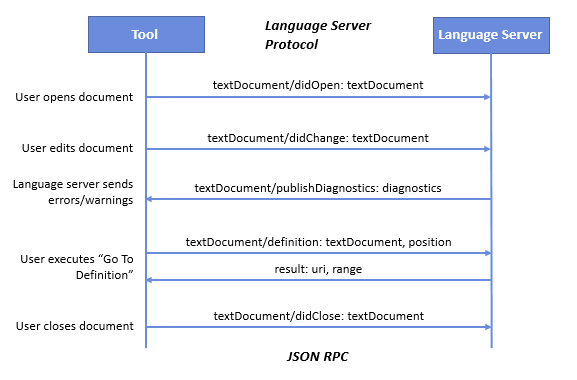
\includegraphics[width=1\textwidth]{img/langServerOverview}
	\caption{Example of the communication between the client and the server}
	\label{fig:langserveroverview}
\end{figure}
The server also gets notified when the user closes a file. An important distinction to make is that whenever the client has opened a file, it resides in memory and the tool maintains it. When it is closed, it simply lies in the file system like any other file. \newline
The communication between the tool and the language server uses JSON RPC v2.0. Language servers can implement an arbitrary subset of features defined in the protocol, so in the first response by the server it details what capabilities it has. \newline
\subsection{Communication Types}
There are two different types to communicate between the client and the server. It's either a notification or a request. 
\paragraph{Notification}
A notification is just a message which can be sent in both directions. But one can't wait for an answer. These types of messages are mostly used to inform the partner that something happened. 
\paragraph{Request}
A request on the other side is a message which will be answered.  
\subsection{Standard Implementation}
Next to custom commands, which are explained in chapter \ref{custom commands} and following, the language server describes a standardized API \cite{protMaster} for features that are useful when working with a language server. The API is designed as a Request / Reply Protocol. Below a list of the implemented Requests is listed, while a detailed description on how the implementation was done can be found in \ref{architecture}. All the structures detailed in this chapter are defined by the protocol. \newline
\paragraph{Message Structure}
The protocol describes how the messages exchanged between the client and the server must be structured. A generic example of a request and a response are as follows:
\textbf{Request}
\begin{lstlisting}[language=json,firstnumber=1]
interface RequestMessage extends Message {

  /**
  * The request id.
  */
  id: number | string;

  /**
  * The method to be invoked.
  */
  method: string;

  /**
  * The method's params.
  */
  params?: any
}
\end{lstlisting}
\textbf{Response}
\begin{lstlisting}[language=json,firstnumber=1]
interface ResponseMessage extends Message {
  /**
  * The request id.
  */
  id: number | string | null;

  /**
  * The result of a request. This can be omitted in
  * the case of an error.
  */
  result?: any;

  /**
  * The error object in case a request fails.
  */
  error?: ResponseError<any>;
}

interface ResponseError<D> {
  /**
  * A number indicating the error type that occurred.
  */
  code: number;

  /**
  * A string providing a short description of the error.
  */
  message: string;

  /**
  * A Primitive or Structured value that contains additional
  * information about the error. Can be omitted.
  */
  data?: D;
}

export namespace ErrorCodes {
  // Defined by JSON RPC
  export const ParseError: number = -32700;
  export const InvalidRequest: number = -32600;
  export const MethodNotFound: number = -32601;
  export const InvalidParams: number = -32602;
  export const InternalError: number = -32603;
  export const serverErrorStart: number = -32099;
  export const serverErrorEnd: number = -32000;
  export const ServerNotInitialized: number = -32002;
  export const UnknownErrorCode: number = -32001;

  // Defined by the protocol.
  export const RequestCancelled: number = -32800;
}
\end{lstlisting}
\paragraph{Data structures}
Next, an overview over the most commonly used data structures used in the protocol is given: \newline
\textbf{Position}
Describes a position, e.g. of a cursor, in a document.
\begin{lstlisting}[language=json,firstnumber=1]
interface Position {
  /**
  * Line position in a document (zero-based).
  */
  line: number;

  /**
  * Character offset on a line in a document (zero-based).
  */
  character: number;
}
\end{lstlisting}
\textbf{Range}
Describes an area in a document which can span multiple lines of text.
\begin{lstlisting}[language=json,firstnumber=1]
interface Range {
  /**
  * The range's start position.
  */
  start: Position;

  /**
  * The range's end position.
  */
  end: Position;
}
\end{lstlisting}
\textbf{Location}
Describes a location inside a resource, such as a line inside a text file.
\begin{lstlisting}[language=json,firstnumber=1]
interface Location {
  uri: DocumentUri;
  range: Range;
}
\end{lstlisting}
\textbf{Diagnostic}
Describes a diagnostic such as an error or a compiler warning.
\begin{lstlisting}[language=json,firstnumber=1]
interface Diagnostic {
  /**
  * The range at which the message applies.
  */
  range: Range;

  /**
  * The diagnostic's severity. Can be omitted. If omitted it is up to the
  * client to interpret diagnostics as error, warning, info or hint.
  */
  severity?: number;

  /**
  * The diagnostic's code. Can be omitted.
  */
  code?: number | string;

  /**
  * A human-readable string describing the source of this
  * diagnostic, e.g. 'typescript' or 'super lint'.
  */
  source?: string;

  /**
  * The diagnostic's message.
  */
  message: string;
}
\end{lstlisting}
\textbf{Server capabilities}
With this data structure, the server can tell the client which features it implements. 
\begin{lstlisting}[language=json,firstnumber=1]
interface ServerCapabilities {
  /**
  * Defines how text documents are synced. Is either a detailed structure defining each notification or
  * for backwards compatibility the TextDocumentSyncKind number.
  */
  textDocumentSync?: TextDocumentSyncOptions | number;
  /**
  * The server provides hover support.
  */
  hoverProvider?: boolean;
  /**
  * The server provides completion support.
  */
  completionProvider?: CompletionOptions;
  /**
  * The server provides signature help support.
  */
  signatureHelpProvider?: SignatureHelpOptions;
  /**
  * The server provides goto definition support.
  */
  definitionProvider?: boolean;
  /**
  * The server provides find references support.
  */
  referencesProvider?: boolean;
  /**
  * The server provides document highlight support.
  */
  documentHighlightProvider?: boolean;
  /**
  * The server provides document symbol support.
  */
  documentSymbolProvider?: boolean;
  /**
  * The server provides workspace symbol support.
  */
  workspaceSymbolProvider?: boolean;
  /**
  * The server provides code actions.
  */
  codeActionProvider?: boolean;
  /**
  * The server provides code lens.
  */
  codeLensProvider?: CodeLensOptions;
  /**
  * The server provides document formatting.
  */
  documentFormattingProvider?: boolean;
  /**
  * The server provides document range formatting.
  */
  documentRangeFormattingProvider?: boolean;
  /**
  * The server provides document formatting on typing.
  */
  documentOnTypeFormattingProvider?: DocumentOnTypeFormattingOptions;
  /**
  * The server provides rename support.
  */
  renameProvider?: boolean;
  /**
  * The server provides document link support.
  */
  documentLinkProvider?: DocumentLinkOptions;
  /**
  * The server provides execute command support.
  */
  executeCommandProvider?: ExecuteCommandOptions;
  /**
  * Experimental server capabilities.
  */
  experimental?: any;
}
\end{lstlisting}

\paragraph{Implemented Requests}
Next, pairs of Request / Responses implemented by this project are listed:
\textbf{Shutdown Request}
The shutdown request is sent from the client to the server. It asks the server to shut down, but to not exit (otherwise the response might not be delivered correctly to the client). There is a separate exit notification that asks the server to exit.

\textbf{Request}
\begin{lstlisting}[language=json,firstnumber=1]
  method: 'shutdown'
  params: void
\end{lstlisting}
\textbf{Response}
\begin{lstlisting}[language=json,firstnumber=1]
result: null
error: code and message set in case an exception happens during shutdown request.
\end{lstlisting}

\textbf{Exit Notification}
A notification to ask the server to exit its process. The server should exit with success code 0 if the shutdown request has been received before; otherwise with error code 1.

\textbf{Notification}
\begin{lstlisting}[language=json,firstnumber=1]
method: 'exit'
params: void
\end{lstlisting}

\textbf{ShowMessage Notification}
The show message notification is sent from a server to a client to ask the client to display a particular message in the user interface.

Notification:
\begin{lstlisting}[language=json,firstnumber=1]
method: 'window/showMessage'
params: ShowMessageParams defined as follows:
interface ShowMessageParams {
  /**
  * The message type. See {@link MessageType}.
  */
  type: number;
	
  /**
  * The actual message.
  */
  message: string;
}
\end{lstlisting}
\textbf{ShowMessage Request}
The show message request is sent from a server to a client to ask the client to display a particular message in the user interface. In addition to the show message notification the request allows to pass actions and to wait for an answer from the client.

Request:
\begin{lstlisting}[language=json,firstnumber=1]
method: 'window/showMessageRequest'
params: ShowMessageRequestParams
\end{lstlisting}
Response:
\begin{lstlisting}[language=json,firstnumber=1]
result: the selected MessageActionItem
error: code and message set in case an exception happens during showing a message.
interface ShowMessageRequestParams {
  /**
  * The message type. See {@link MessageType}
  */
  type: number;
	
  /**
  * The actual message
  */
  message: string;
	
  /**
  * The message action items to present.
  */
  actions?: MessageActionItem[];
}
\end{lstlisting}

\textbf{DidChangeConfiguration Notification}

A notification sent from the client to the server to signal the change of configuration settings.

Notification:
\begin{lstlisting}[language=json,firstnumber=1]
method: 'workspace/didChangeConfiguration',
params: DidChangeConfigurationParams defined as follows:
interface DidChangeConfigurationParams {
  /**
  * The actual changed settings
  */
  settings: any;
}
\end{lstlisting}

\textbf{DidOpenTextDocument Notification}

The document open notification is sent from the client to the server to signal newly opened text documents. The document's truth is now managed by the client and the server must not try to read the document's truth using the document's Uri.

Notification:
\begin{lstlisting}[language=json,firstnumber=1]
method: 'textDocument/didOpen'
params: DidOpenTextDocumentParams defined as follows:
interface DidOpenTextDocumentParams {
  /**
  * The document that was opened.
  */
  textDocument: TextDocumentItem;
}
\end{lstlisting}

\textbf{DidChangeTextDocument Notification}

The document change notification is sent from the client to the server to signal changes to a text document. In 2.0 the shape of the params has changed to include proper version numbers and language ids.

Notification:
\begin{lstlisting}[language=json,firstnumber=1]
method: 'textDocument/didChange'
params: DidChangeTextDocumentParams defined as follows:
interface DidChangeTextDocumentParams {
  /**
  * The document that did change. The version number points
  * to the version after all provided content changes have
  * been applied.
  */
  textDocument: VersionedTextDocumentIdentifier;
	
  /**
  * The actual content changes.
  */
  contentChanges: TextDocumentContentChangeEvent[];
}
\end{lstlisting}

\textbf{DidCloseTextDocument Notification}

The document close notification is sent from the client to the server when the document got closed in the client. The document's truth now exists where the document's Uri points to (e.g. if the document's Uri is a file Uri the truth now exists on disk).

Notification:
\begin{lstlisting}[language=json,firstnumber=1]
method: 'textDocument/didClose'
params: DidCloseTextDocumentParams defined as follows:
interface DidCloseTextDocumentParams {
  /**
  * The document that was closed.
  */
  textDocument: TextDocumentIdentifier;
}
\end{lstlisting}

\textbf{PublishDiagnostics Notification}

Diagnostics notification are sent from the server to the client to signal results of validation runs.

Notification:
\begin{lstlisting}[language=json,firstnumber=1]
method: 'textDocument/publishDiagnostics'
params: PublishDiagnosticsParams defined as follows:
interface PublishDiagnosticsParams {
  /**
  * The URI for which diagnostic information is reported.
  */
  uri: DocumentUri;
	
  /**
  * An array of diagnostic information items.
  */
  diagnostics: Diagnostic[];
}
\end{lstlisting}
\textbf{Completion Request}

The Completion request is sent from the client to the server to compute completion items at a given cursor position. Completion items are presented in the IntelliSense user interface. If computing full completion items is expensive, servers can additionally provide a handler for the completion item resolve request ('completionItem/resolve'). This request is sent when a completion item is selected in the user interface. A typically use case is for example: the 'textDocument/completion' request doesn't fill in the documentation property for returned completion items since it is expensive to compute. When the item is selected in the user interface then a 'completionItem/resolve' request is sent with the selected completion item as a param. The returned completion item should have the documentation property filled in.

Request:
\begin{lstlisting}[language=json,firstnumber=1]
method: 'textDocument/completion'
params: TextDocumentPositionParams
\end{lstlisting}
Response:
\begin{lstlisting}[language=json,firstnumber=1]
result: CompletionItem[] | CompletionList
/**
* Represents a collection of [completion items](#CompletionItem) to be presented
* in the editor.
*/
interface CompletionList {
  /**
  * This list it not complete. Further typing should result in recomputing
  * this list.
  */
  isIncomplete: boolean;
  /**
  * The completion items.
  */
  items: CompletionItem[];
}
\end{lstlisting}

\textbf{Go to Definition Request}

The go to definition request is sent from the client to the server to resolve the definition location of a symbol at a given text document position.

Request:
\begin{lstlisting}[language=json,firstnumber=1]
method: 'textDocument/definition'
params: TextDocumentPositionParams
\end{lstlisting}

Response:
\begin{lstlisting}[language=json,firstnumber=1]
result: Location | Location[]
error: code and message set in case an exception happens during the definition request.
Registration Options: TextDocumentRegistrationOptions
\end{lstlisting}

\textbf{Find References Request}

The references request is sent from the client to the server to resolve project-wide references for the symbol denoted by the given text document position.

Request:
\begin{lstlisting}[language=json,firstnumber=1]
method: 'textDocument/references'
params: ReferenceParams defined as follows:
interface ReferenceParams extends TextDocumentPositionParams {
	context: ReferenceContext
}
interface ReferenceContext {
  /**
  * Include the declaration of the current symbol.
  */
  includeDeclaration: boolean;
}
\end{lstlisting}
Response:
\begin{lstlisting}[language=json,firstnumber=1]
result: Location[]
error: code and message set in case an exception happens during the reference request.
Registration Options: TextDocumentRegistrationOptions
\end{lstlisting}

\textbf{Code Action Request}

The code action request is sent from the client to the server to compute commands for a given text document and range. These commands are typically code fixes to either fix problems or to beautify/refactor code.

Request:
\begin{lstlisting}[language=json,firstnumber=1]
method: 'textDocument/codeAction'
params: CodeActionParams defined as follows:
/**
* Params for the CodeActionRequest
*/
interface CodeActionParams {
  /**
  * The document in which the command was invoked.
  */
  textDocument: TextDocumentIdentifier;
	
  /**
  * The range for which the command was invoked.
  */
  range: Range;
	
  /**
  * Context carrying additional information.
  */
  context: CodeActionContext;
}

/**
* Contains additional diagnostic information about the context in which
* a code action is run.
*/
interface CodeActionContext {
  /**
  * An array of diagnostics.
  */
  diagnostics: Diagnostic[];
}
\end{lstlisting}
Response:
\begin{lstlisting}[language=json,firstnumber=1]
result: Command[] defined as follows:
error: code and message set in case an exception happens during the code action request.
Registration Options: TextDocumentRegistrationOptions
\end{lstlisting}

\textbf{Code Lens Request}

The code lens request is sent from the client to the server to compute code lenses for a given text document.

Request:
\begin{lstlisting}[language=json,firstnumber=1]
method: 'textDocument/codeLens'
params: CodeLensParams defined as follows:
interface CodeLensParams {
  /**
  * The document to request code lens for.
  */
  textDocument: TextDocumentIdentifier;
}
\end{lstlisting}
Response:
\begin{lstlisting}[language=json,firstnumber=1]
result: CodeLens[] defined as follows:
/**
* A code lens represents a command that should be shown along with
* source text, like the number of references, a way to run tests, etc.
*
* A code lens is _unresolved_ when no command is associated to it. For performance
* reasons the creation of a code lens and resolving should be done in two stages.
*/
interface CodeLens {
  /**
  * The range in which this code lens is valid. Should only span a single line.
  */
  range: Range;
	
  /**
  * The command this code lens represents.
  */
  command?: Command;
	
  /**
  * A data entry field that is preserved on a code lens item between
  * a code lens and a code lens resolve request.
  */
  data?: any
}
error: code and message set in case an exception happens during the code lens request.
\end{lstlisting}

\textbf{Code Lens Resolve Request}

The code lens resolve request is sent from the client to the server to resolve the command for a given code lens item.

Request:
\begin{lstlisting}[language=json,firstnumber=1]
method: 'codeLens/resolve'
params: CodeLens
\end{lstlisting}

Response:
\begin{lstlisting}[language=json,firstnumber=1]
result: CodeLens
error: code and message set in case an exception happens during the code lens resolve request.
\end{lstlisting}

\textbf{Rename Request}

The rename request is sent from the client to the server to perform a workspace-wide rename of a symbol.

Request:
\begin{lstlisting}[language=json,firstnumber=1]
method: 'textDocument/rename'
params: RenameParams defined as follows
interface RenameParams {
  /**
  * The document to format.
  */
  textDocument: TextDocumentIdentifier;

  /**
  * The position at which this request was sent.
  */
  position: Position;

  /**
  * The new name of the symbol. If the given name is not valid the
  * request must return a [ResponseError](#ResponseError) with an
  * appropriate message set.
  */
  newName: string;
}
\end{lstlisting}
Response:
\begin{lstlisting}[language=json,firstnumber=1]
result: WorkspaceEdit describing the modification to the workspace.
error: code and message set in case an exception happens during the rename request.
Registration Options: TextDocumentRegistrationOptions
\end{lstlisting}


\subsection{Custom Extensions}\label{custom commands}
The following chapters will explain in detail which additions were made, comparing to the standard messages of the language server protocol. This additions were implemented either with requests or notifications. The standard allows to send these type of messages, with a name and a payload.
They were needed to have features like installing Dafny, restarting the DafnyServer or updating the queue size. All features which are not normal IDE features. 
Therefore to support a new IDE all the \textbf{Server $\longrightarrow$ Client} have to be implemented and handled in the new client.

\subsubsection{Notification Server $\longrightarrow$ Client}

\textbf{ERROR}
This message is sent if something happens which the user should be informed about. Examples would be that the compilation failed or the DafnyServer wasn't found. \newline

\textbf{WARNING}
This message is sent if the mono path is specified but mono is in the path. \newline

\textbf{INFO}
Info messages appear quite often to inform the user about the current progress. \newline

\textbf{dafnymissing}
This informs the client that the verification of the DafnyServer has failed or that there is a newer version available. The text is sent as a additional parameter.  \newline

\textbf{queueSize}
This message updates the queue size number in the status bar on the right side. \newline

\textbf{serverStarted}
This message contains two additional parameters, which are also important for the status bar. They are the PID and the version of the started DafnyServer instance. It is sent after the dependencies have been checked and the DafnyServer have been spawned. \newline

\textbf{activeVerifiyingDocument}
As soon as a verification is sent to the DafnyServer, the client is informed to show if the user has this file open. \newline

\textbf{verificationResult}
All verification results are sent to the server, for fast access times. Switching from one file to the other updates the verification result on the left side based on these results. \newline

\textbf{changeServerStatus}
All states from the server are also sent to the client to update the status bar. \newline

\textbf{ready}
This message is sent directly after the serverStarted message to inform the DafnyClientProvider that verification requests can now be sent. \newline

\textbf{progress}
Used to inform users about progress during downloading and extracting of Dafny. This notification has also the following data attached: domain, current, total\newline

\subsubsection{Request Server $\longrightarrow$ Client}
There are no requests which are sent from the server to the client. 

\subsubsection{Notification Client $\longrightarrow$ Server}

\textbf{verify}
This notification contains the document which has to be verified. On the server it is put into a queue and the result is sent via verificationResult. \newline

\textbf{counterExample}
This message is sent directly after the serverStarted message to inform the DafnyClientProvider that verification requests can now be sent. \newline


\subsubsection{Request Client $\longrightarrow$ Server}

\textbf{reset}
Resets the DafnyServer on the Server and restarts it. This can be useful if the caching of the DafnyServer is not working correctly anymore. \newline

\textbf{compile}
Sends a request containing only the Uri to the corresponding file. Starts the Dafny.exe with parameters to generate either a dll or an exe. After the compilation, it returns possible errors, if it is executable and a message.\newline

\textbf{install}
Executes first an uninstallation if Dafny is installed. Afterwards downloads Dafny and extracts it. Additionally the install folder is sent in the response to update the configuration. \newline

\textbf{uninstall}
First stops the running instance and then removes the current Dafny installation. \newline

\textbf{dotgraph}
Generates a flow graph for the file sent. Returns as the generation has been completed. \newline


\subsection{Commands}
Commands are specified in the client and can trigger different actions. One can specify names for them and register shortcuts from them. The server can also send commands. This was needed for example to show references, because there was a transformation necessary, so that the arguments are the right types, before the command is executed. The method signature was not the same as in the language server protocol specification. 

\subsubsection{Commands Server $\longrightarrow$ Client}
\textbf{dafny.showReferences}
Used by CodeLens to show references of methods. The method transforms the arguments and forward them to the \textbf{editor.action.showReferences} command. 

\textbf{dafny.editText}
Used by rename to do text modifications. Should process all text edits which are sent. 

\subsubsection{Commands Client}

\textbf{dafny.restartDafnyServer}
Restarts the DafnyServer with the "Reset Request".\newline

\textbf{dafny.installDafny}
This command is used to trigger the install request, either by a context menu or a shortcut. 
First it runs the uninstallDafny command to be sure that there is no running instance. Afterwards downloads the latest version from GitHub. This process is either executed from an upgrade message, not installed message or can be executed manually. 
See \nameref{fig:Version upgrade available} for a better overview over the installation process. \newline

\textbf{dafny.uninstallDafny}
First stops any DafnyServer instance and deletes all files which belongs to Dafny. \newline

\textbf{dafny.showReferences}
This is used to show references from CodeLenses. Unfortunately the command editor.action.showReferences can not be used directly, because of some internal problems. To solve that, all parameters have to be copied and passed to this command. \newline

\textbf{dafny.editText}
Mainly used for all refactoring to change text in the active text document. \newline

\textbf{dafny.compile}
Shortcut: ctrl+shift+b or shift+apple+b
\newline
Compile the current document \newline

\textbf{dafny.compileAndRun}
Shortcut: F5
\newline
Compile the current document, and if there is a "Main Method", start the corresponding executable. \newline

\textbf{dafny.showDotGraph}
Shortcut: F6
\newline
Generates a flow graph out of the current file. Displays all the graphs in a second view. \newline

\textbf{dafny.showCounterExample}
Shortcut: F7
\newline
Calculates the counter example for the current file. \newline

\textbf{dafny.hideCounterExample}
Shortcut: F8
\newline
Hide the counter example in the current file.  \newline


\subsection{Process overview}
The following graphs should help to understand how the main processes are run through.
In the beginning, the client always connects to the language server (left out in the last picture). As soon as this connection is established, different events are registered on both sides. The next step is that the client sends the configuration, which is the entry point to start the verification if Dafny is installed. Afterwards it starts to differ depending on the case. 

\subsubsection{Startup process}
If Dafny is installed, the version is queried, to perform afterwards a version check on GitHub. If the latest version in installed, the DafnyServer is started and the client informed. After the client received the "Ready" message, additional listeners are registered like save, document change and close. All the events which now can trigger a verification of the current document. If a verification should be performed, the language server sends the request towards the DafnyServer. The output is analyzed and the sent back to the client. The server status is sent on each of these steps as well.    
\begin{figure}[H]
	\centering
	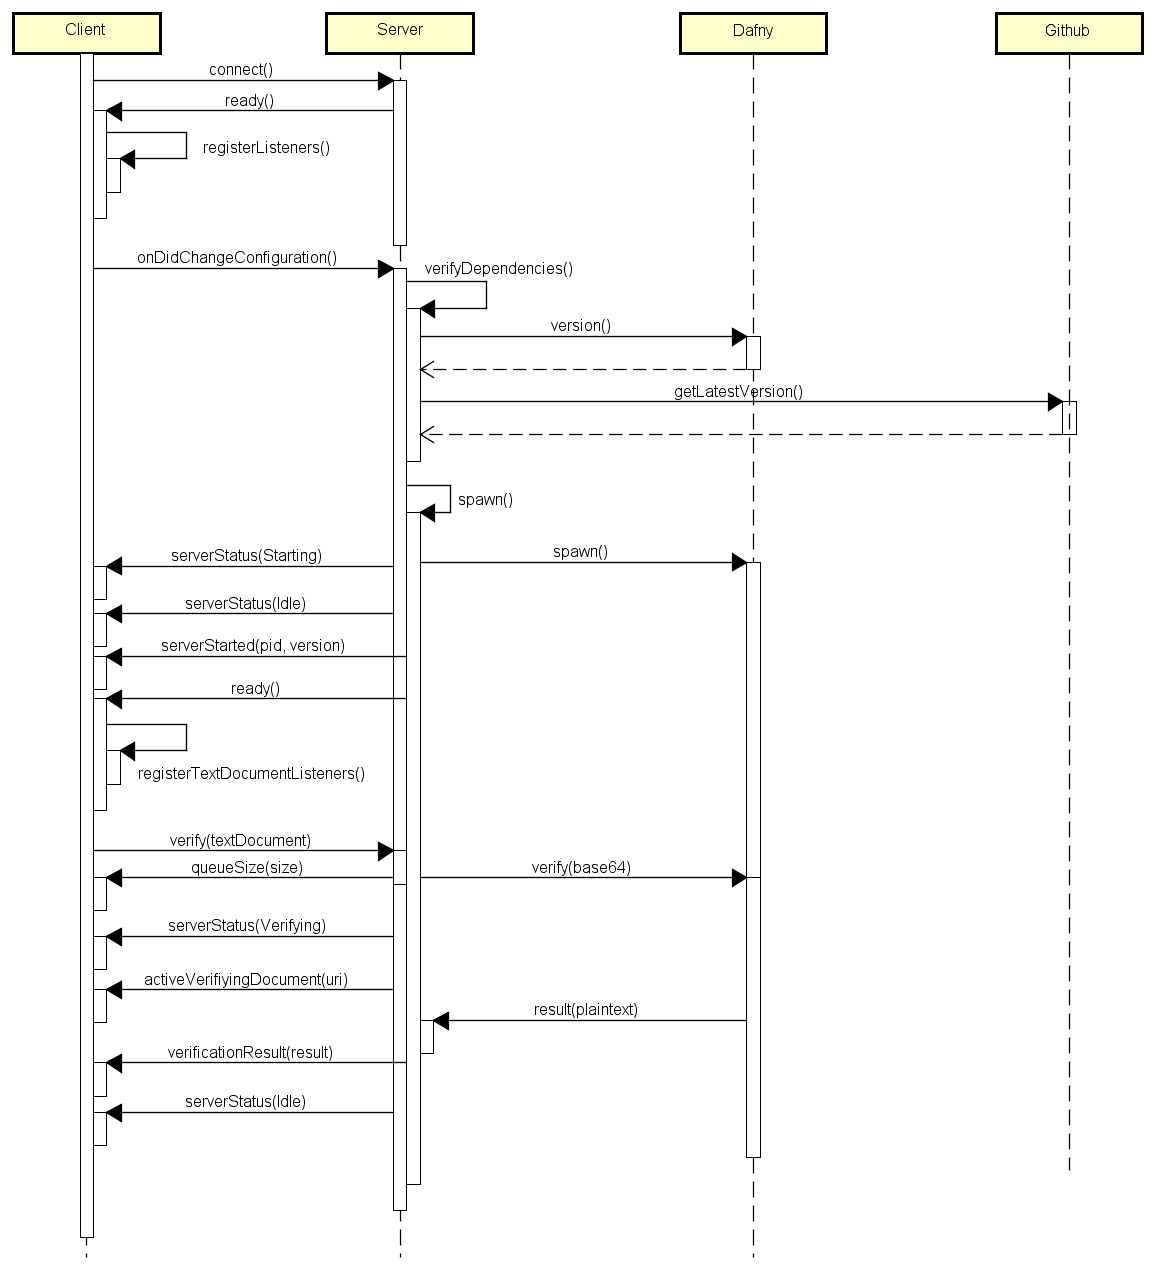
\includegraphics[width=1\textwidth]{img/DafnyStartupFull}
	\caption{DafnyServer startup}
	\label{fig:DafnyServer startup}
\end{figure}

\subsubsection{Not installed}
If Dafny is not installed, the user is informed that Dafny can not be started and asks if it should be installed. It either fails if the DafnyServer can not be started or the verb version is not implemented. If the answer is yes, the flow will continue in the next graphic on install()
\begin{figure}[H]
	\centering
	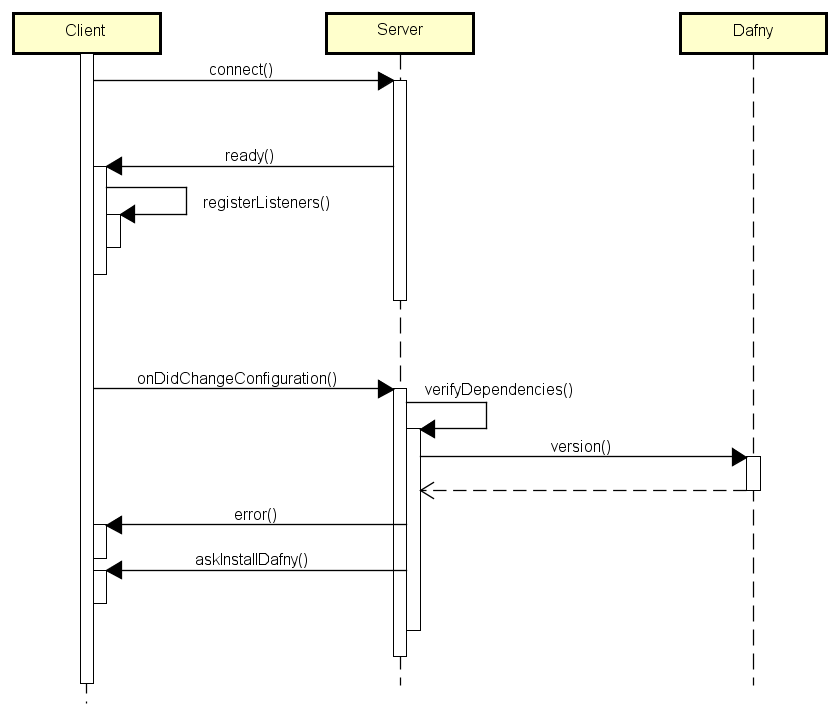
\includegraphics[width=1\textwidth]{img/DafnyNotInstalled}
	\caption{Dafny not installed}
	\label{fig:Dafny not installed}
\end{figure}

\subsubsection{Installation - Upgrade available}
After the version of Dafny is known and the comparison with the release information of GitHub shows that there is a newer release available. In that case the DafnyServer is started normally, but the user is also informed that there is a newer version. If the answer is yes, the installation starts. The first step is to stop the DafnyServer, if it is active, to perform after that an uninstallation regardless if Dafny was installed. Afterwards, depending of the platform, the correct release is downloaded from GitHub. During that step, progress notifications are sent to the client (not visible in the graphic). As soon as the download is finished the archive is extracted again with progress information. The last step is to do start over and do the verification again. 
\begin{figure}[H]
	\centering
	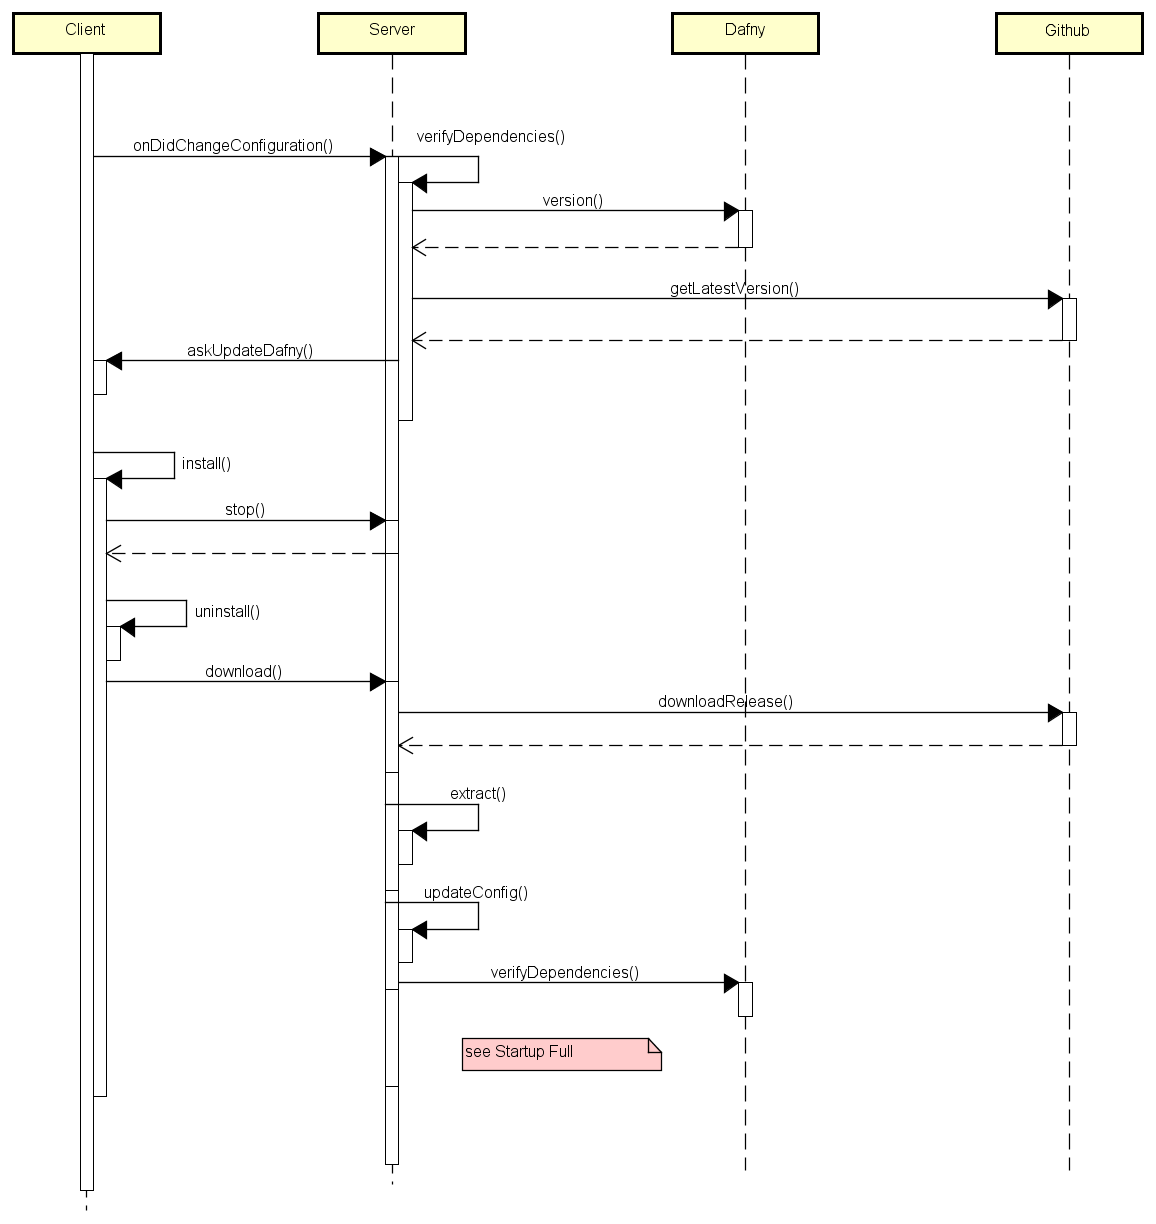
\includegraphics[width=1\textwidth]{img/DafnyVersionUpgrade}
	\caption{Version upgrade available}
	\label{fig:Version upgrade available}
\end{figure}




\section{Architecture and Implementation} \label{architecture}
This chapter documents the architecture and the implementation of the plugin.

\subsection{Features} \label{features}
This chapter details the different features that were implemented during the project. They are mostly language agnostic features that were implemented according to the language server protocol to offer a richer IDE experience. The backbone of the language server protocol is the interface IConnection. When the plugin is started, an instance of this interface is established which allows communication from the client (the IDE) to the server (the plugin / the language server). On this connection, generic requests and replies can be sent and received, but the language server protocol also offers defined messages for common IDE features. Further insight into this can be won in \ref{langserver} \newline
For instance, if the plugin wants to support rename element, it must provide a callback to the onRenameRequest on the connection. The input to this callback usually is the information needed to answer the request, typically a document and a position in it. The language server is then free in its implementation on how to answer these requests. \newline
Usually this is done by a so called provider, a class which implements at least one method that can answer such a request. This method is then registered as a callback to that element when the plugin is initialized.\newline
This project also chose this approach, for every IDE feature a provider was implemented, which carries out the task of answering such a request. The providers themselves are heavily based on the symbol service. Both the providers and the symbol service are explained below.\newline 
\begin{figure}[H]
	\centering
	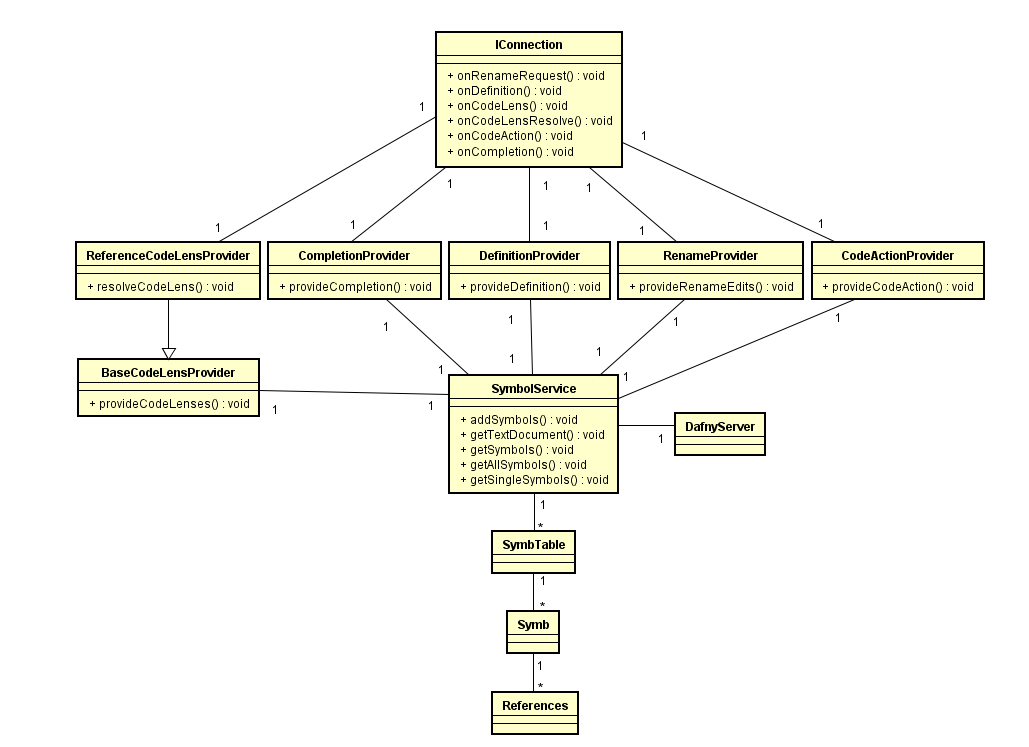
\includegraphics[width=1\textwidth]{img/featureArchitecture}
	\caption{How the IDE-features are integrated into the language server}
	\label{fig:featurearchitecture}
\end{figure}
\subsubsection{CodeLenses} \label{codelenses}
CodeLenses are Visual Studio Code a feature which is also common to many other IDEs. The idea is to display meta information about certain pieces of codes, for instance classes and methods. In Visual Studio Code this is done  by adding an additional line of text to the editor wherever a codeLense should  be placed. \newline
\begin{figure}[H]
	\centering
	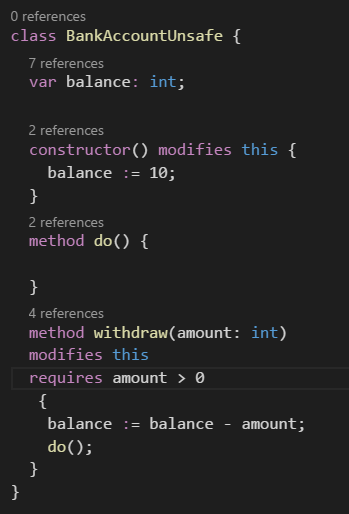
\includegraphics[width=0.5\textwidth]{img/codelensesClosed}
	\caption{Code Lenses used with Dafny}
	\label{fig:codelensesclosed}
\end{figure}
It was decided to display codeLenses for classes, methods (including constructors) and fields, since they tend to have a wide scope in the code bases \newline
A second consideration was which information should be displayed in a codeLens. When codeLenses are language specific and do not for instance stem from a plugin which displays code metrics or similar, usually references and usages of the element are displayed. It was decided to display this information also for the Dafny plugin. CodeLenses also allow commands to be executed when clicked upon, a logical conclusion is to implement go to reference when a reference in a codeLens is clicked.\newline
Since the tasks of finding the elements which need a codeLens and constructing the codelens itself are very different, the implementations were separated in a base class and a child class. The base class answers the onCodeLens request of the connection and the child class then answers the onCodeLensResolve request. The reasoning for this lies in possible future expansion, as maybe additional information should be displayed in a codeLens. This can be done in an own child class, the produced codeLenses (which stem from the same placeholder codeLens) then are automatically merged by Visual Studio Code. This design was also inspired by the GoLang Plugin \cite{godef}. 
\begin{figure}[H]
	\centering
	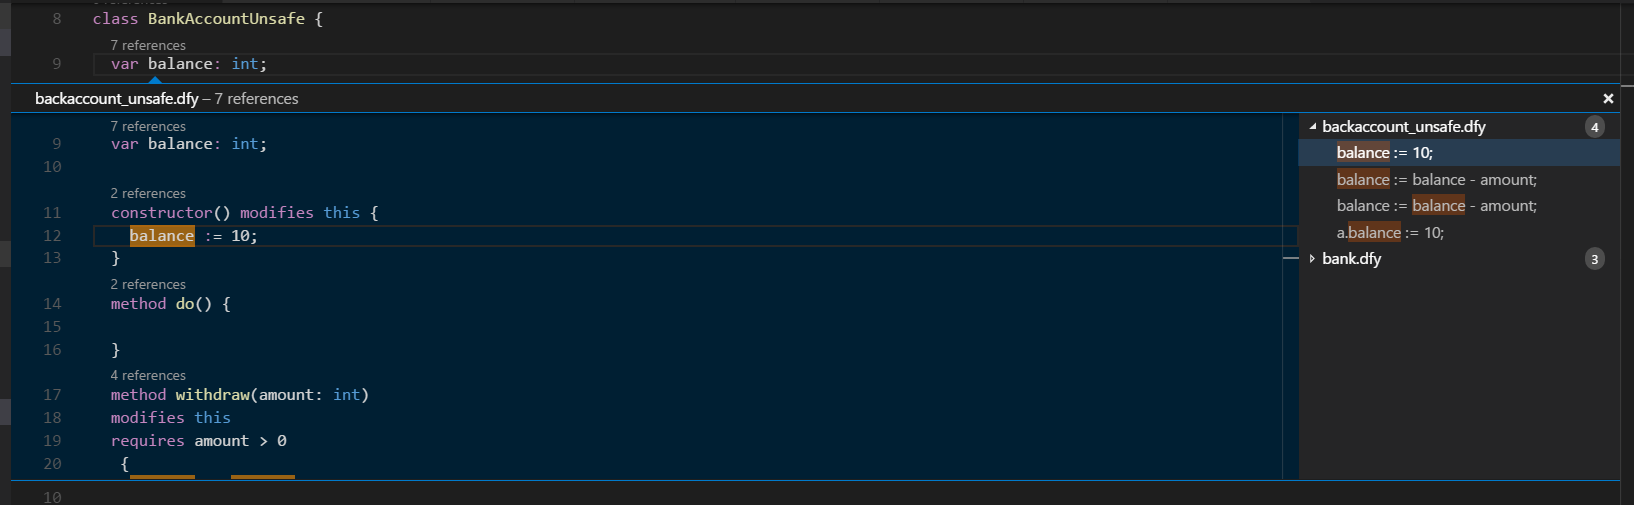
\includegraphics[width=1\textwidth]{img/codelensesExpanded}
	\caption{Expanded codeLens showing the references to the field balance}
	\label{fig:codelensesexpanded}
\end{figure}
The only challenging aspect when implementing this feature is that references can't be determined via a simple text search, since different classes could have members with the same name. To only display unambiguous references, the search has to be done via the fully qualified domain name of the symbol. Since information about references is needed often, all references are determined by the DafnyServer and returned together with the symbol information to the symbol service. This allows for simple processing in the language server itself and the references are updated in real time, since the symbol service refreshes the symbols for a file when it is changed. Off course also the file path belonging to the file in which the reference occurs is returned by the symbol service. This is needed when a reference is in  file external to the defining one and the go to reference command is invoked.\newline
When given locations of the references, it is possible to let Visual Studio Code highlight them in the preview window which opens when a codeLens is expanded. Visual Studio Code also groups references according to the file path in the location, so the programmer gets to see a map of all references ordered by containing file to the right of the preview window and can quickly navigate to them.
\subsubsection{Code Completion} \label{codecompletion}
Code completion has become a standard feature for IDEs. Usually, when the programmer starts typing, a little popup appears in which the programmer can choose options that complete the code he is currently writing. \newline
\begin{figure}[H]
	\centering
	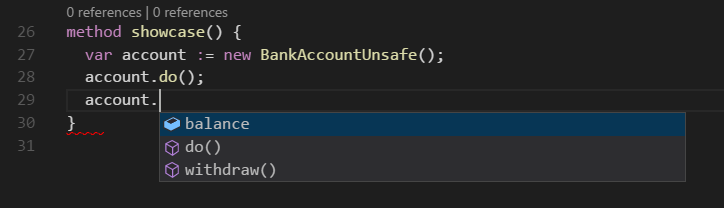
\includegraphics[width=1\textwidth]{img/codeCompletionOverview}
	\caption{Popup with completion options}
	\label{fig:codecompletionoverview}
\end{figure}
There are several different considerations when implementing code completion in a language server. The first one is to define which typed characters should trigger a completion request. Ideally, an IDE supports the programmer with completion regardless of the current context. Next to performance, another reason to narrow down the trigger selection is that not all contexts warrant meaningful suggestions for completion. In this project, a pragmatic approach was chosen where completion is triggered when ever a "." is typed, a situation where the programmer usually wants to access a member of an element. Since there is usually a designator present before the ".", there is also enough knowledge present about the current context to offer meaningful options. \newline
In order to support this, the symbol service stores all variable declarations so the plugin knows about the type of all expressions that can be followed by a ".". The completion request comes with a position in the current file as an argument, so the first task is to resolve the expression and find out the fully qualified name of each element. The language server then searches the symbol service for all members that are defined in the class with that fully qualified name and sends them back as completion suggestions. \newline
Visual Studio Code then handles all further actions, for instance, once the popup is displayed and the programmer continues to type, it removes all suggestions that don't start with the typed characters. It is also possible to display further information regarding the suggestions. The plugin already details if the completion is a field or a method, which Visual Studio Code provides  separate icons for. When the suggestion is a method, the preconditions, if any, are also displayed, so the programmer already knows the constraints he is writing under. \newline
 \begin{figure}[H]
	\centering
	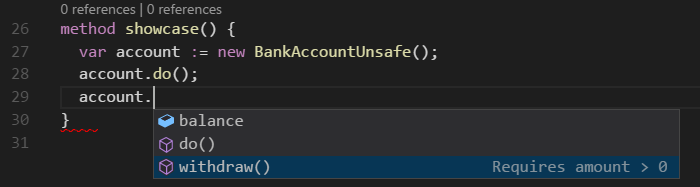
\includegraphics[width=1\textwidth]{img/codeCompletionMethod}
	\caption{Suggestion displaying precondition}
	\label{fig:codecompletionmethod}
\end{figure}
The implementation is straightforward, as the symbol service already provides ways to resolve the fully qualified name of an expression and if it as an alias for an element of a class, all therein defined methods and fields can simply be collected. The method and field symbols in the symbol services also contain all additional information which is displayed in the popup. Possible improvements in the completion feature would be support of built in methods and functions and also offer context aware completion when the programmer starts to type an identifier. 
\subsubsection{Go to Definition} \label{gotodefinition}
Another common feature is go to definition. It enables the programmer to quickly jump to the definition of a code element he is currently working with in order to gain further insight about it. This can usually be done either via a hot key for the current cursor position or an option when opening the context menu via a right click, Visual Studio Code offers both ways.\newline
\begin{figure}[H]
	\centering
	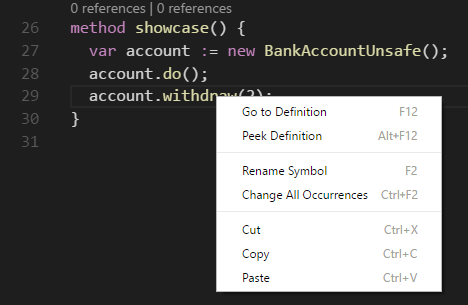
\includegraphics[width=0.5\textwidth]{img/goToDefinition}
	\caption{The Definition Features}
	\label{fig:gotodefinition}
\end{figure}
The language server protocol offers an on definition request, which has the URI of the file and the position for which a definition is requested as parameters. The plugin then first tries to resolve the word at the position which could lead to a definition. When a word could be resolved, the plugin tries to determine if the expression is an alias for an element of a class or if it stands for an access of a member of one. If this is the case, the fully qualified name of the symbol can be determined via the symbol service, as it stores information about all definitions and declarations. The plugin than finds the unambiguous definition via the fully qualified name and responds with the location of that definition. This also works if the definition is in an external file in the same workspace. \newline
If, for whatever reason, the fully qualified name cannot be determined, the plugin tries to match the selected word with any symbol cached in the symbol service. This approach only works as best effort though, as different classes could defines methods with the same name for example. If no match is found at all, no definition is provided. \newline
Visual Studio Code offers two options when searching for definitions, either go to definition which immediately opens the returned location in an editor or peek definition, which shows the definition in a little popup. \newline
 \begin{figure}[H]
	\centering
	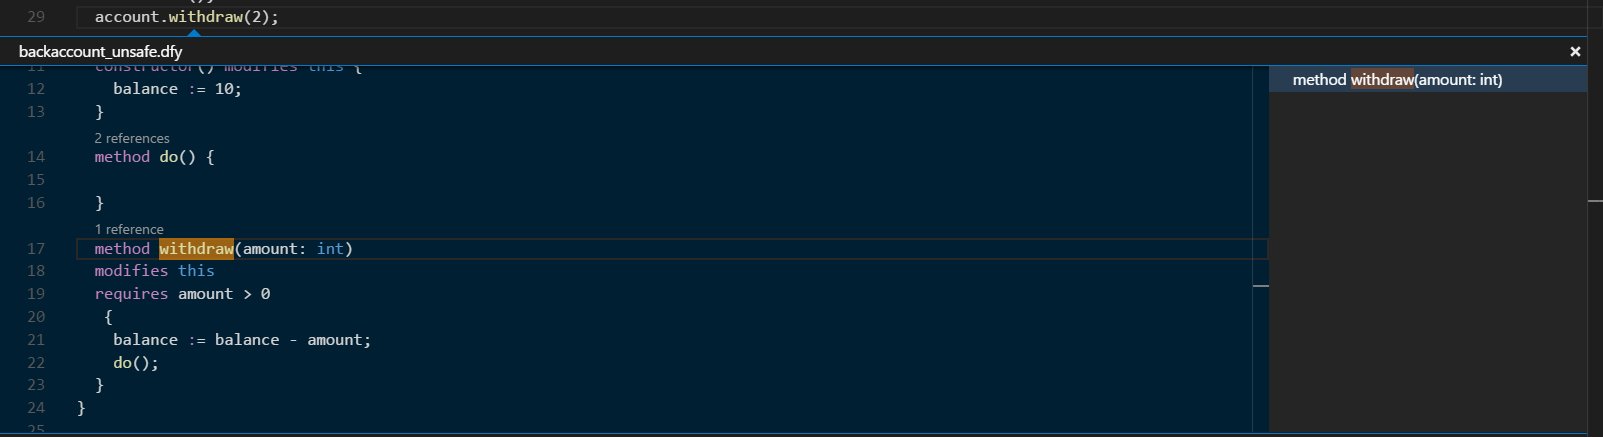
\includegraphics[width=1\textwidth]{img/goToDefinitionPeek}
	\caption{Overlay of peeked definition}
	\label{fig:gotodefinitionpeek}
\end{figure}
Extensions to this feature could be a context aware heuristic when a fully qualified name cannot be determined where for instance the current and nearby files are preferred when searching for definitions. Also, when polymorphism comes into play and the actual implementation cannot be determined, at the current state the first possibility is returned. The could be enhanced by offering all possible definitions.
\subsubsection{Rename Element} \label{renameelement}
Rename element is a feature essential to refactoring. It allows to quickly make code better readable. Visual Studio Code offers built in support for renaming either via a hot key or the context menu. \newline
The language server protocol, as with many other features, offers a request for renaming with the URI of the file in which the command was invoked and the position belonging to the command. Additionally, the new name of the element should have is also given as an argument. The protocol expects a collection of textedit commands, which entail an URI of file, and ranges in that file which should be replaced with a word. \newline
As often with the language server protocol, the first step when implementing the feature is to determine the element at the position which is given as an argument. When the position can be resolved to a meaningful word, the plugin tries to determine if it is either an alias for an element of a class, or a member of class, for instance a field or a method. If it can do so with absolutely certainty, the fully qualified name of that element is obtained. The next step is trivial, since the symbol service already caches all references to a symbol, information which it gained through the DafnyServer. The plugin can simply build textedits out of all references, since the reference already contain all necessary information such as the containing file and their position therein. This therefor also works across multiple files which reference the same element, as long they are open in the same workspace. Those textedits are then returned from the language server to Visual Studio Code, which does all the actual replacing. \newline
  \begin{figure}[H]
 	\centering
 	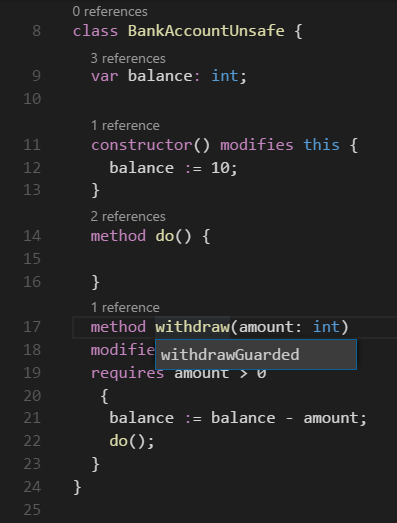
\includegraphics[width=0.5\textwidth]{img/rename}
 	\caption{Renaming an element in Visual Studio Code}
 	\label{fig:rename}
 \end{figure}
Since this feature actually changes code that is worked with, the implementation must be very robust and failsafe. Thus, it was implemented very defensive. It the location of a requested renaming cannot be resolved to a meaningful word, the request is ended without dictating any changes. The same holds if a word can resolved, but it cannot be matched to a fully qualified name. In this case, possible references could be ambiguous, so no action should be taken. To further limit the possibility for failure, the scope for this feature is very small. The current implementation only allows for renaming of class members such as fields and methods, since these can be resolved with absolute certainty.\newline
When extending this feature, it would be beneficial to also be able to rename local variables for instance. To do this, the symbol information which the DafnyServer returns to the symbol service would have to be enriched with detailed scope information to allow being able to exactly say which regions are prone to renamings and which are not. 
\subsubsection{Quick Fixes} \label{quickfixes}
Quick Fixes are a versatile feature in IDEs which basically allow to do any manipulation to code. Usually they are offered as reactions to diagnostics which were provided earlier. A simple example would be implementing a spell checker this way, offering to replace a wrongly written word with the correct spelling. \newline
Since this feature has no clear implementation guideline, and the plugin designer can implement almost anything that he likes this way, this was an obvious place to implement Dafny specific feature in the plugin.\newline
They way this works in Visual Studio Code is that when the diagnostic stage for the file has been completed, where all things such as compiler warnings or custom warnings are generated, a new request is fired at the language server. This request holds a collection of all diagnostics on the current file and the language server is free to either do nothing are provide commands for some diagnostics in the collection which often aim to resolve the shortcomings detailed by the diagnostic. \newline
  \begin{figure}[H]
	\centering
	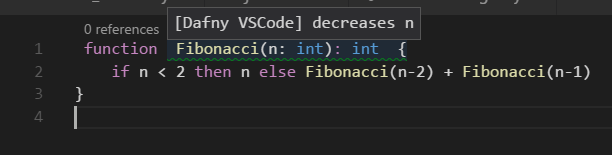
\includegraphics[width=0.7\textwidth]{img/diagnostic}
	\caption{Visual Studio Code displays a diagnostic}
	\label{fig:diagnostic}
\end{figure}
The current stand of the projects offers three code fixes to resolve Dafny specific diagnostics. \newline
The first one is a common situation where a programmer fails to capture his intention that an expression should either decrease or increase when working with recursion or loops. It can also be the case that an expression must always evaluate into a certain range, this is for instance the case when an expression that is used as an index to an array is not constant within a loop. The remedy is simple, a decrease / increase guard with the expression in question must be added at the correct location. In case an expression must be within a certain range, the same intent can be written as an invariant. \newline
  \begin{figure}[H]
	\centering
	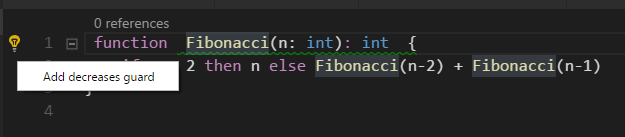
\includegraphics[width=0.7\textwidth]{img/decreaseGuard}
	\caption{Offering a code fix to add a guard}
	\label{fig:decreaseguard}
\end{figure}
This situation can easily be identified through the message within the diagnostic, since Dafny always gives this message in the same format. The expression that has to be decreased can also easily be parsed out of this message. The placement of the guard is a little more difficult, the implementation tries to find the first block in which the variables used in the expression are not in scope anymore. The guard is then inserted before the block containing the first usage. \newline
  \begin{figure}[H]
	\centering
	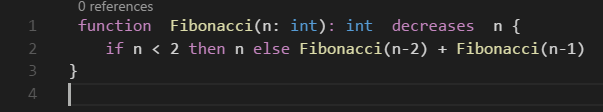
\includegraphics[width=0.7\textwidth]{img/decreaseGuardApplied}
	\caption{Program after the code fix}
	\label{fig:decreaseguardapplied}
\end{figure}
The second code fix the plugin offers is very similar, but this time the constraint is that an object may be null when it should not. The situation again is easily detected through the message in the diagnostic, and also the expression which should not be null can be parsed through it.
  \begin{figure}[H]
	\centering
	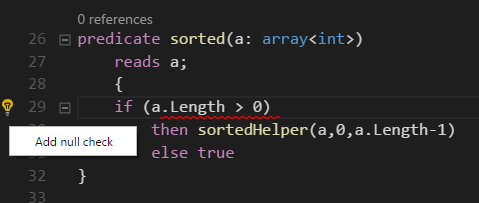
\includegraphics[width=0.7\textwidth]{img/nullCheck}
	\caption{It should be made sure that an element is not null}
	\label{fig:nullcheck}
\end{figure}
Also the search for the insertion position works very similarly. It then inserts the constraint in form of a precondition to the surrounding element. \newline
  \begin{figure}[H]
	\centering
	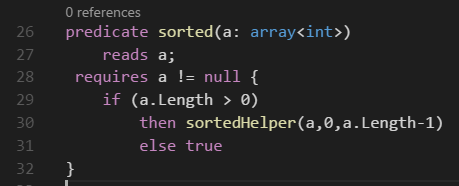
\includegraphics[width=0.7\textwidth]{img/nullCheckApplied}
	\caption{The precondition has been added}
	\label{fig:nullcheckapplied}
\end{figure}
The third code fix is to implement bound checking for expressions which are used to index an array. This can either take the form of a precondition, if the expression is constant within the block of code in question, are the form of an invariant if the expression is dynamic (for instance in a loop).
The remedy is to apply the bound checking either through preconditions or invariants, depending on the context.
  \begin{figure}[H]
	\centering
	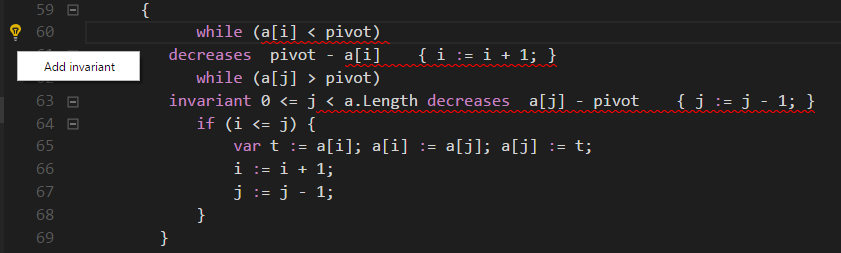
\includegraphics[width=1\textwidth]{img/indexOutRangeDiag}
	\caption{The expression may be out of range}
	\label{fig:indexOutOfRange}
\end{figure}
The first difficult part is to find the expression that is used as an index, as well as the identifier which stands for the array. Both is done through pattern matching on the code file in regard to the position of the diagnostic. Next it must be decided if preconditions or invariants should get generated, for this there must be knowledge about the context, e.g. if the expression is static in the current block. This is done via the information saved in the symbol service and also some pattern matching. \newline
Finally, the invariant or the preconditions must be inserted into the correct place. For this, all identifiers used in the expressions must be matched against their declaration, in order place the guards when already all symbols have been declared. \newline
  \begin{figure}[H]
	\centering
	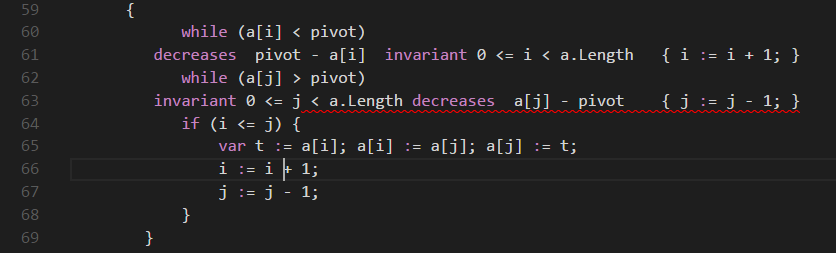
\includegraphics[width=1\textwidth]{img/indexChecked}
	\caption{Invariants for the loop were generated}
	\label{fig:indexInBound}
\end{figure}
At the current stand, only these three code fixes are implemented, the possible extensions are legion. One idea is to insert code that decreases a given expression when Dafny can't prove that an expression always decreases in a block were such a decrease clause was declared.\newline
\subsubsection{Counter Examples}
A useful features which also can provide a huge benefit, is to show an example which violates the contract, if the program can't be verified. Especially if the method is large with many branches, it can be very difficult to see how an example could look like which is not correct regarding the contract. \newline
Z3 verifies mathematical expression by trying to find a proof for the negation of the proof. That means if it finds a proof the program is not correct. But more important Z3 finds a assignment for the different variables which violate the contract. This knowledge can be used to show a counterexample in Visual Studio Code. The only big step is to translate the counterexample, which is called model in Z3, back into something that can be matched with the Dafny program. Fortunately this is already done in the DafnyProvider in Boogie. Additionally, to get only the necessary information out of it and also to show the values of class fields, the translation needed to be extended. A new server verb counterExample was introduced, which returns a counter example which is JSON encoded. Thereby it was possible to show assignments of the variables on each line in Visual Studio Code. \newline
This is a easy example of a invalid method which should return the ABS, but misses to handle negative numbers correctly. 
\begin{figure}[H]
	\centering
	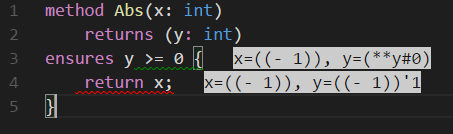
\includegraphics[width=0.7\textwidth]{img/counterModel}
	\caption{Counter Example is shown in Visual Studio Code}
	\label{fig:counterModel}
\end{figure}
Below is a more complex example of a class. The goal of the withdraw method is to prevent the balance to be below zero. Therefore the postcondition "ensures balance >= 0" exists. With help of the counter example it becomes clear that the amount is to big. It is bigger than zero though, but this precondition is wrong. It should be that the amount must be smaller than the balance. On the first line it shows that the balance is 2275 and the amount 2276 in the counter example. This results into the balance being negative after the subtraction. 
\begin{figure}[H]
	\centering
	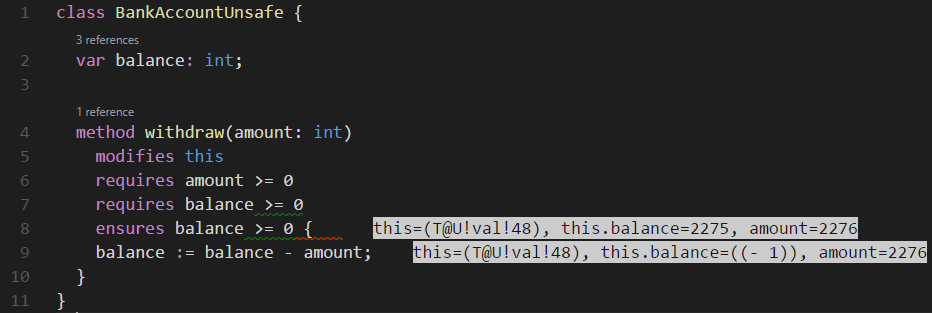
\includegraphics[width=1\textwidth]{img/counterModelBank}
	\caption{Counter Example inside a class}
	\label{fig:counterModelBank}
\end{figure}

\subsection{Environment}\label{environment}
This chapter details the underlying structure of the plugin which provides a basis to implement the individual concrete features.

\subsubsection{Symbol Service}\label{symbolservice}
The different features often need detailed information about symbols and their relations. A symbol table is a data structure used by a compiler to keep track of scope / binding information about names. These names are used in the source program to identify the various program elements, like variables, constants, procedures, and the labels of statements.\cite[239]{compiler} \newline
With regard to performance, but also to reduce overhead it was decided to implement a symbol service in the language server part of the plugin. It's main goal is to cache a subset of the symbol table of the compiler, such that features which need information about names in the code can use the symbol service to gain this insight without having to invoke the compiler every time a lookup has to be performed or each feature having to handle the information caching separately \newline
Since compilation is a heavy task, results should be cached efficiently. There is a trade off here though with the validity of the symbols, since if they are cashed too long, they don't represent the code anymore. The solution chosen is a lazy loading approach, meaning whenever a component queries the service the first time, the symbols are loaded and cached for the first time. This is usually done through by codeLenses, since they need the symbol information and they are created every time a file is opened right at the start. To make sure that no unnecessary loads are performed, the symbol table for each document is stored alongside a hash of the content of the document. Before sending a new request to DafnyServer, a comparison of the hashes is done to ascertain that the file really has changed. In future, this would also allow efficient caching by using histories of symbol tables when actions are undone. Next to the symbol table, it also stores the supplied text document itself, allowing for quick text manipulation if the content has not changed when loading the symbols.\newline
The next consideration was on how to store the symbol table and which information should be saved. The fields used are mostly needed to either determine which kind of symbol it is, where its scope is, its fully qualified name and relationships in form of references are also stored. This lead to the following data structure that is stored in the symbol service, the example is simplified for better readability: \newline
\newline\newline
\textbf{Symbol Tables: }
\begin{lstlisting}[language=json,firstnumber=1]
[
 {
  fileName: "filepathInUriFormat",
  hash: -483616355,
  symbols: [
   {
    call: null,
    column: 5,
    document: "filepathInUriFormat",
    end: Range(8, 12),
    ensures: [...],
    line: 8,
    module: "module",
    name: "balance",
    parentClass: "BankAccountUnsafe",
    position: 96,
    range(start, end),
    References: [
     {
      column: 4,
      document: "filepathInUriFormat",
      end: Range(11, 11),
      line: 11,
      methodName: "balance",
      position: 154,
      range: Range(start, end),
      referencedName: "balance"
     },
     ...
    ],
    requires: [...],
    start: Range(8, 5),
    symbolType: "Field"
   },
   ...
  ]
 },
 ...
]
\end{lstlisting}

The possible symbol types that are stored are defined as follows:
\begin{lstlisting}[language=json,firstnumber=1]
{
 Unknown,
 Class,
 Method,
 Function,
 Field,
 Call,
 Declaration	
}

\end{lstlisting}
The symbol table offers the following API to obtain symbols: \newline
\paragraph{addSymbols(doc: Textdocument, symbols: SymbolTable, forceAddition: boolean=false): void} This saves the supplied symbol table and associates it with the text document given. The default behavior is to get a new symbol table from the DafnyServer anyway and compare if they have changed. If so, the never one is chosen and persisted. If the parameter forceAddition is set to true, the symbol table is stored even though it might be out of date, a new version is not queried.

\paragraph{getTextDocument(uri: string): TextDocument} If the service has cached a text document specified by the Uri supplied, it returns it.

\paragraph{getSymbols(doc: TextDocument): Promise<SymbolTable[]>} Returns all the symbol tables that are stored in the symbol service. Optionally, a text document can be given as an argument. If the symbols to this document are not cached, then they are queried from the DafnyServer. Since this is an asynchronous operation, the return type is a promise of symbol tables. This method is useful when actions have to be done across the whole workspace.

\paragraph{getAllSymbols(doc: TextDocument): Promise<Symbol[]>} Similar to the method above, but the result is already flattened to an array of symbols across the whole code base. This is useful when it is not important to work with the symbols on a file per file basis.

\paragraph{getSingleSymbols(doc: TextDocument): Promise<SymbolTable>} This method allows for gaining the symbols for a single text document. If they are not cached yet, the service queries the Dafny Server for it, stores the result and then returns it. Since this operation is asynchronous, the return type is a promise.
\newline
When querying the the DafnyServer, the server defensively starts the communication with it by supplying the symbol verb, the file path and content for which it wants symbols on stdout. It then waits on the socket for a response, and if it is well formed and contains the queried symbols, the JSON returned by the server is parsed and the new symbol elements are constructed out of the JSON, which are then saved in the service. \newline
When there is an error, for instance a connection error, or there was a compilation error which prevents the building of a symbol table, the service deals with the error and just keeps, if it has any, the old symbol table of the file, so that the data is always in the most consistent state possible. Since compilation errors or connection errors are signaled to the user, the service listens until the broken elements have been repaired and then queries the server again for the symbols. \newline
Parsing of a successful response is also done conservatively, meaning that if an important property on for instance a method symbol is missing, this symbol is not stored, although all other valid symbols from that batch are stored. This allows for the maximum of analysis with only partly correct data. \newline
An improvement to the symbol service could be to do the caching more cleverly, for instance ignoring white space changes. A trade off in this area is that the calculations to decide if an update should be made could be more expensive then the update itself, so this should be monitored closely. Also when more and more complex refactoring and analysis should be done with the plugin, the data structure stored must probably be expanded. The extreme would be to save the whole AST in the symbol service which off course would be an overkill. Also here a balance thusly must be found between information richness and scope. Another consideration could be to optimize the lazy loading approach, for instance draw on a simple heuristic which files might be opened soon and load the symbols for them preemptively\newline



\section{System Setup}
This chapter details the infrastructure that was used in this project. It includes the local setup on the developer machines as well as all remote infrastructure such as continuous integration and project management tools. 
\subsection{Local setup}
\begin{itemize}
	\item TexStudio 2.12
	\item Visual Studio Code 1.9
	\item Git
\end{itemize}
\subsection{Server setup}
\begin{itemize}
	\item Jira
	\item Bamboo
	\item NodeJS
	\item SonarQube
	\item Postgres
\end{itemize}
\subsection{Continuous Integration}
To ensure that the code quality is high and the code is working as expected, all commits trigger automated builds of the respective project. A commit to the documentation repository executes a job which creates a file out of the \LaTeX sources. This document is then copied to the \emph{wwwroot} directory, which then can be downloaded from the project homepage. Commits to the vscode-dafny repository will result in a build and a complete run of all tests on the three environments afterwards. Therefore remote agents are installed on Ubuntu and OSX , which test the plugin on these operation system.  Additionally SonarQube is used to find bugs and bad practices as early as possible. The last repository which triggers a bamboo job is the project homepage. The latest version is built and deployed when a commit is performed. 
\begin{figure}[H]
	\centering
	\includegraphics[width=0.9\textwidth]{img/ci}
	\caption{Server Setup}
	\label{fig:Server setup}
\end{figure}
\section{Testing}
This section details what was tested in this project and how the testing environment was set up.
\subsection{Test specification}
\subsubsection{Unit Tests}
Visual Studio Code plugins can be tested with standard Javascript testing frameworks like Mocha or Jasmine, if they do not use any features of Visual Studio Code itself. This allows to test core logic without the need to run tests inside VS Code.
\subsubsection{Integration Tests}
Visual Studio Code extensions which require VS Code API can be tested with help of a special instance of Visual Studio Code. Inside this instance, the extension can use the full API and tests can execute commands like creating a new file, entering a character, using auto completion and verifying if the extension works as expected.   
\subsubsection{Test overview}
To verify that the Dafny Visual Studio Code Plugin is working as expected, it has to be properly tested. Two possibilities exist. Either automatic unit / integration tests or manual testing. The best would be to test everything automatically. Unfortunately this is not possible, since although the Visual Studio Code Test API provides a rich set of methods, there is no direct access to the file system or a possibility to wait for certain tasks to finish. For this reason some tests have to be performed manually, especially use cases which install Dafny and rely heavily on scripts. On the other hand, if all automatic tests fail, it is mostly a clear signal that something with the server is not okay. So the automatic tests also verify if the DafnyServer is working correctly. During development it is also quite easy to verify certain features on the fly. 
Below one first finds what is tested and how, followed by a table, which explains how the individual use cases are tested and guides for manual testing. 
\subsubsection{System Tests}
As discussed in the last chapter, not everything can be easily tested, so the test scope has to be restricted. The following table shows which system component are tested and how.
\rowcolors{2}{gray!25}{white}
\begin{longtable}{ p{0.3\textwidth} | p{0.2\textwidth} | p{0.4\textwidth} }
\rowcolor{gray!50}
	\textbf{Topic} & \textbf{Tested} & \textbf{Description}\\
	Installation of Dafny plugin & Manually & Manual installation of Dafny and setting of base path   \\
	Automatic installation of Dafny & Manually & Easier to validate that base path is set correctly and all files exists \\
	Uninstallation of Dafny & Manually & Verify on file system level\\
	Communication DafnyServer and Dafny plugin & Manually + Automatically & Test if output from DafnyServer is correctly parsed and displayed\\
	Restart DafnyServer task & Manually & Check if a new PID is used and the other is stopped\\
	Local queue & Manually & DafnyServer can be paused in Visual Studio Code and queuing can be checked \\
	Syntax highlighting & Manually & Look at example code \\
	Verification on typing & Manually & Easy to test manually\\
	Snippets & Manually & Check if snippets are working\\
	File verification & Automatically & As a .dfy is opened the DafnyServer is started and the file verified \\
	Counter Model & Automatic & Verifies that the counter model is correctly sent from the DafnyServer over the server to the client \\
	\caption{System Tests}
	\label{tab:System Tests}
\end{longtable}


\subsubsection{Basic tests}
If the Dafny plugin is installed, the following procedure is expected inside Visual Studio Code.  
\begin{itemize}
	\item The Dafny language is available
	\item .dfy is associated with the Dafny plugin
	\item Asks to install Dafny, if no DafnyServer is found 
	\item Starts the DafnyServer if a .dfy is opened
	\item Verification status of a .dfy file is shown
	\item Assertion errors are reported
\end{itemize}

\subsubsection{Detailed manual tests}
The following paragraphs explain how a certain feature can be tested manually, which steps have to be performed and what the expected result should be.

\paragraph{Manual installation}
\textbf{\newline Steps:}
\begin{enumerate}
	\item Uninstall the plugin and remove Dafny (/home/.dafny or C:/Users/\%Username\%/.dafny)
	\item Remove the entry "dafny.basePath" from the user configuration file 
	\item Restart Visual Studio Code - There should be an error that Dafny is not installed
	\item Install Dafny from \href{https://github.com/FunctionalCorrectness/dafny-microsoft/releases}{https://github.com/FunctionalCorrectness/dafny-microsoft/releases}
	\item Set "dafny.basePath" to the extracted archive location
	\item Restart Visual Studio Code
	\item Open the file simpleTest.dfy
	\item Execute "Dafny: RestartServer" task
\end{enumerate}
\textbf{\newline Expected:}
The DafnyServer should be started and the file verified. This can be seen in the status bar. On the right side, there should be the PID of the DafnyServer and on the left side the status "Verified"

\paragraph{Status change}
\textbf{\newline Steps:}
\begin{enumerate}
	\item Open the file invalidAsserts.dfy
	
\end{enumerate}
\textbf{\newline Expected:}
The server should first start and afterwards the status should display "Verifiying". After the DafnyServer verified the program, the status should have been changed to "Not Verified" and multiple asserts are marked red. 

\paragraph{Server crash}
\textbf{\newline Steps:}
\begin{enumerate}
	\item Open the file simpleTest.dfy
	\item The server should be started and the file verified
	\item Kill the DafnyServer process
\end{enumerate}
\textbf{\newline Expected:}
The server should restart automatically, with a corresponding message shown inside Visual Studio Code. 

\paragraph{Local queue}
\textbf{\newline Steps:}
\begin{enumerate}
	\item Open the file simpleTest.dfy
	\item The server should be started and the file verified
	\item Open Visual Studio Code and attach the debugger to the DafnyServer process
	\item Set a breakpoint in the verify method
	\item Change an assert in the simpleTest.dfy 
	\item Visual Studio Code should break at the breakpoint
	\item Open more files
\end{enumerate}
\textbf{\newline Expected:}
The queue size should be getting bigger and bigger as new files are opened. After the breakpoint is removed and the debugger detached, the queue size should decrease. 

\paragraph{Verification on typing}
\textbf{\newline Steps:}
\begin{enumerate}
	\item Open the file simpleTest.dfy
	\item Change an assert that it does not hold (in under 0.7 seconds)
\end{enumerate}
\textbf{\newline Expected:}
After 0.7 seconds (default value) the file should be verified and the error should be displayed 

\paragraph{Automatic installation}
\textbf{\newline Steps:}
\begin{enumerate}
	\item Uninstall the Server with "Dafny: Uninstall DafnyServer" task
	\item Restart Visual Studio Code - There should be an error that Dafny is not installed
	\item Open the file simpleTest.dfy
	\item Install Dafny with the task "Dafny: Install DafnyServer" 
\end{enumerate}
\textbf{\newline Expected:}
Dafny should be downloaded, extracted, started and the file verified. See UC1, UC2, UC3 Expected

\paragraph{Uninstallation}
\textbf{\newline Steps:}
\begin{enumerate}
	\item Uninstall the Server with "Dafny: Uninstall DafnyServer" task
\end{enumerate}
\textbf{\newline Expected:}
Dafny should be uninstalled from the system. /home/.Dafny or \%AppData\%/Roaming/Dafny should be empty.

\paragraph{Snippets}
\textbf{\newline Steps:}
\begin{enumerate}
	\item Open the source code file snippets/dafny.json and remember a prefix from the list
	\item Enter the prefix 
	\item Press Enter
\end{enumerate}
\textbf{\newline Expected:}
The snippet should be inserted and can be edited

\paragraph{Auto completion for identifiers}
Auto completion can be tested with the Visual Studio Code Test API. For this, a file is loaded with a set of methods. Afterwards, some test checks if the existing methods are considered for auto completion. In addition, more refactoring tests will be performed under this use case. 


\appendix

\listoffigures
\addcontentsline{toc}{section}{\listfigurename}

\listoftables
\addcontentsline{toc}{section}{\listtablename}
\printbibliography[heading=bibintoc]
%\section{Anhang}
[Placeholder]
\end{document}
